\title{GPIB to USB}
\documentclass[12pt]{article}
\usepackage{listings}
\usepackage[english]{babel}
\usepackage[utf8x]{inputenc}
\usepackage{amsmath}
\usepackage{graphicx}
\usepackage[colorinlistoftodos]{todonotes}

\begin{document}

\begin{titlepage}

\newcommand{\HRule}{\rule{\linewidth}{0.5mm}} % Defines a new command for the horizontal lines, change thickness here

\center % Center everything on the page
%----------------------------------------------------------------------------------------
%	LOGO SECTION
%----------------------------------------------------------------------------------------


\includegraphics[width=50mm]{tu.jpg} % Include a department/university logo - this will require the graphicx package
 
%----------------------------------------------------------------------------------------


%----------------------------------------------------------------------------------------
%	HEADING SECTIONS
%----------------------------------------------------------------------------------------

\textsc{\LARGE Tribhuwan University}\\[1.5cm] % Name of your university/college
\textsc{\Large Instrumentation II}\\[0.5cm] % Major heading such as course name
\textsc{\large Hardware Project Report}\\[0.5cm] % Minor heading such as course title

%----------------------------------------------------------------------------------------
%	TITLE SECTION
%----------------------------------------------------------------------------------------

\HRule \\[0.2cm]
{ \huge \bfseries GPIB TO USB}\\[0.4cm] % Title of your document
\HRule \\[1.5cm]
 
%----------------------------------------------------------------------------------------
%	AUTHOR SECTION
%----------------------------------------------------------------------------------------

%\begin{minipage}{0.4\textwidth}
%\begin{flushleft} \large
%\emph{Author:}\\
%Sujit \textsc{Maharjan} \\
%Shishir \textsc{Aditya Gautam} \\
%Shreya \textsc{Agarwal} % Your name
%\end{flushleft}
%\end{minipage}
~
%\begin{minipage}{0.4\textwidth}
%\begin{flushright} \large
%\emph{Supervisor:} \\
%Dr. James \textsc{Smith} % Supervisor's Name
%\end{flushright}
%\end{minipage}\\[2cm]

% If you don't want a supervisor, uncomment the two lines below and remove the section above
\Large \emph{Author:}\\
Sujit \textsc{Maharjan} (070BEX443) \\
Sujal \textsc{Dhungana} (070BEX442)\\
Shreya \textsc{Agarwal} (070BEX441)\\
Sujita \textsc{Chaudhary} (070BEX444)\\[1cm]

%----------------------------------------------------------------------------------------
%	DATE SECTION
%----------------------------------------------------------------------------------------

{\large \today}\\[1cm] % Date, change the \today to a set date if you want to be precise


\vfill % Fill the rest of the page with whitespace

\end{titlepage}

\section{Acknowledgement}

First and foremost, we would like express our gratitude to the IOE (Institute Of Engineering), Central Campus Pulchowk, Department of Electronics and Computer Engineering for the wonderful opportunity to explore the wonderful field of automation and circuit design. The corporation and the support provided by the campus has been fruitful for the successful completion of the case study.
\par
We would also like to extend our gratitude to Mr. Dinesh Baniya kshetri, Subject Teacher for  his effort to share his knowledge on the subject matter which enabled us to take our first starting step on this Project. We would also like to thank  Mr. Sumit Maharjan who is currently doing his Masters in Natural Language Programming in Tohokyo University, Sendai, Japan for his guidance in using LaTeX.\par
We are also grateful to many hard working people who have provided us with software resources like latex, Emacs, Google drives/docs, git which enhanced our teams ability to collaborate and create this report with ease which we would not feel with the lack of any of these technologies.
\par
Also extending the thanks to our friends who have heartily involved in any discussion sharing ideas and help whenever possible.

\newpage



\tableofcontents
\newpage
\renewcommand{\thesection}{\arabic{section}} 
\section{Introduction}


The primary function of microprocessor is to accept data from input devices such as keyboard and A/D converters, read instructions from memory, process data accordingly to the instructions, and send the results to output devices such as LEDs, printers and video monitors.In the case of this project we accept data from oscillator  computer through GPIB to USB connectors.    These input and output devices are called peripherals or I/Os. Designing the logic circuits (hardware) and writing instructions (software) to enable the microprocessor to communicate with these peripherals is called interfacing, and the logic circuits are called I/O ports of interfacing devices.\par
Interfacing requires the following:
\begin{itemize}
\item Electrical and Mechanical Interfacing\par
Electrical Compatibility ensures that two devices have similar voltage and architecture.\par
Mechanical Compatibility ensures that the connectors fit properly.
\item Data Compatibility\par
Data Compatibility ensures that two or more devices agree upon a common protocol.
\item Timing Compatibility\par
If the transmitter and receiver agree on the data transfer rate or data reception rate then information can be exchanged easily.\par
If the data transfer rate is different between transmission and receiver, handshaking signals are required to maintain data transfer compatibility.
\end{itemize}



\newpage

\section{Objective}
\begin{itemize}
\item To get familiarized  with the design, simulation of circuits.
\item To get familiarized  with creation of printed circuit boards (PCB).
\item To get familiarized  with driver and application software development.
\item To get familiarized  with IEEE-488 connector. 
\end{itemize}
\newpage
\section{Devices Used}
\subsection{IEEE-488}
IEEE-488 is a short-range digital communications 8-bit parallel multi-master interface bus specification. IEEE-488 was created as HP-IB (Hewlett-Packard Interface Bus) and is commonly called GPIB (General Purpose Interface Bus). It has been the subject of several standards.\par 

Although originally created in the late 1960s to connect together automated test equipment, it also had some success during the 1970s and 80s as a peripheral bus for early microcomputers, notably the Commodore PET. Newer standards have largely replaced IEEE-488 for computer use, but it still sees some use in the test equipment field.
\subsubsection{ Characteristics}
IEEE-488 is an 8-bit, electrically parallel bus. The bus employs sixteen signal lines — eight used for bi-directional data transfer, three for handshake, and five for bus management — plus eight ground return lines.\par 

Every device on the bus has a unique 5-bit primary address, in the range from 0 to 30 (31 total possible addresses).\par 

The standard allows up to 15 devices to share a single physical bus of up to 20 meters total cable length. The physical topology can be linear or star (forked). Active extenders allow longer buses, with up to 31 devices theoretically possible on a logical bus.\par 

Control and data transfer functions are logically separated; a controller can address one device as a “talker” and one or more devices as “listeners” without having to participate in the data transfer. It is possible for multiple controllers to share the same bus; but only one can be the "Controller In Charge" at a time.\par 

In the original protocol, transfers use an interlocked, three-wire ready–valid–accepted handshake. The maximum data rate is about one megabyte per second. The later HS-488 extension relaxes the handshake requirements, allowing up to 8 Mbyte/s. The slowest participating device determines the speed of the bus.\par 
\subsubsection{Connectors}
IEEE-488 specifies a 24-pin Amphenol-designed micro ribbon connector. Micro ribbon connectors have a D-shaped metal shell, but are larger than D-subminiature connectors. They are sometimes called "Centronics connectors" after the 36-pin micro ribbon connector Centronics used for their printers.\par 

One unusual feature of IEEE-488 connectors is they commonly use a "double-headed" design, with male on one side, and female on the other. This allows stacking connectors for easy daisy-chaining. Mechanical considerations limit the number of stacked connectors to four or fewer, although a workaround involving physically supporting the connectors may be able to get around this.\par 

They are held in place by screws, either UTS (now largely obsolete) or metric M3.5×0.6 threads. Early versions of the standard suggested that metric screws should be blackened to avoid confusion with the incompatible UTS threads. However, by the 1987 revision this was no longer considered necessary because of the prevalence of metric threads.\par 

The IEC-60625 standard prescribes the use of 25-pin D-subminiature connectors (the same as used for the parallel port on IBM-PCs). This connector did not gain significant market acceptance against the established 24-pin connector.\par 
\begin{figure}[!h]
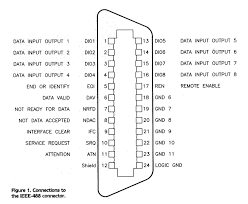
\includegraphics[width=3in]{images}
\caption{Pin Diagram of IEEE-488}
\centering
\end{figure}
\newpage
\subsection{USB (UNIVERSAL SERIAL BUS)}
USB, short for Universal Serial Bus, is an industry standard developed in the mid-1990s that defines the cables, connectors and communications protocols used in a bus for connection, communication, and power supply between computers and electronic devices.It is currently developed by the USB Implementers Forum.\par 

USB was designed to standardize the connection of computer peripherals (including keyboards, pointing devices, digital cameras, printers, portable media players, disk drives and network adapters) to personal computers, both to communicate and to supply electric power. It has become commonplace on other devices, such as smartphones, PDAs and video game consoles. USB has effectively replaced a variety of earlier interfaces, such as parallel ports, as well as separate power chargers for portable devices.\par 
\begin{figure}[!h]
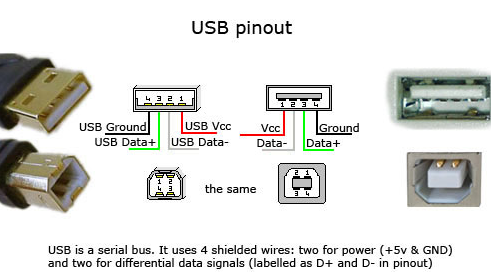
\includegraphics[width=3in]{usb}
\centering
\caption{Pin Diagram of USB}
\end{figure}
\subsection{ATMEL AVR}
The AVR is a modified Harvard architecture 8-bit RISC single-chip microcontroller, which was developed by Atmel in 1996. The AVR was one of the first microcontroller families to use on-chip flash memory for program storage, as opposed to one-time programmable ROM, EPROM, or EEPROM used by other microcontrollers at the time.\par 
\subsubsection{features}
\begin{itemize}
\item Multifunction, bi-directional general-purpose I/O ports with configurable, built-in pull-up resistors
\item Multiple internal oscillators, including RC oscillator without external parts
\item  Internal, self-programmable instruction flash memory up to 256 kB (384 kB on XMega)
\item  In-system programmable using serial/parallel low-voltage proprietary interfaces or JTAG
\item  Optional boot code section with independent lock bits for protection
\item  On-chip debugging (OCD) support through JTAG or debugWIRE on most devices
\item  The JTAG signals (TMS, TDI, TDO, and TCK) are multiplexed on GPIOs. These pins can be configured to function as JTAG or GPIO depending on the setting of a fuse bit, which can be programmed via ISP or HVSP. By default, AVRs with JTAG come with the JTAG interface enabled.
\item debug WIRE uses the /RESET pin as a bi-directional communication channel to access on-chip debug circuitry. It is present on devices with lower pin counts, as it only requires one pin.
\item  Internal data EEPROM up to 4 kB
\item  Internal SRAM up to 16 kB (32 kB on XMega)
\item  External 64 kB little endian data space on certain models, including the Mega8515 and Mega162.
\item  The external data space is overlaid with the internal data space, such that the full 64 kB address space does not appear on the external bus and accesses to e.g. address 010016 will access internal RAM, not the external bus.
\item  In certain members of the XMega series, the external data space has been enhanced to support both SRAM and SDRAM. As well, the data addressing modes have been expanded to allow up to 16 MB of data memory to be directly addressed.
\item AVRs generally do not support executing code from external memory. Some ASSPs using the AVR core do support external program memory.
\item 8-bit and 16-bit timers
\item  PWM output (some devices have an enhanced PWM peripheral which includes a dead-time generator)
\item Input capture that record a time stamp triggered by a signal edge
\item Analog comparator
\item 10 or 12-bit A/D converters, with multiplex of up to 16 channels
\item 12-bit D/A converters
\item A variety of serial interfaces, including
\item I²C compatible Two-Wire Interface (TWI)
\item Synchronous/asynchronous serial peripherals (UART/USART) (used with RS-232, RS-485, and more)
\item Serial Peripheral Interface Bus (SPI)
\item Universal Serial Interface (USI): a multi-purpose hardware communication module that can be used to implement an SPI, I2C or UART interface.
\item Brownout detection
\item Watchdog timer (WDT)
\item Multiple power-saving sleep modes
\item Lighting and motor control (PWM-specific) controller models
\item CAN controller support
\item USB controller support
\item Proper full-speed (12 Mbit/s) hardware \& Hub controller with embedded AVR.
\item Also freely available low-speed (1.5 Mbit/s) (HID) 
\item bitbanging software emulations
\item Ethernet controller support
\item LCD controller support
\item Low-voltage devices operating down to 1.8 V (to 0.7 V for parts with built-in DC–DC upconverter)
\item picoPower devices
\item DMA controllers and "event system" peripheral communication.
\item Fast cryptography support for AES and DES
\end{itemize}
\subsection{PRINTED CIRCUIT BOARD (PCB)}
PCB is an acronym for printed circuit board. It is a board that has lines and pads that connect various points together. In the picture above, there are traces that electrically connect the various connectors and components to each other. A PCB allows signals and power to be routed between physical devices.

\subsubsection{Design}
Initially PCBs were designed manually by creating a photomask on a clear mylar sheet, usually at two or four times the true size. Starting from the schematic diagram the component pin pads were laid out on the mylar and then traces were routed to connect the pads. Rub-on dry transfers of common component footprints increased efficiency. Traces were made with self-adhesive tape. Pre-printed non-reproducing grids on the mylar assisted in layout. To fabricate the board, the finished photomask was photolithographically reproduced onto a photoresist coating on the blank copper-clad boards.\par 
 Modern PCBs are designed with dedicated layout software, generally in the following steps:
\begin{itemize}
\item Schematic capture through an electronic design automation (EDA) tool.
\item Card dimensions and template are decided based on required circuitry and case of the PCB.
\item The positions of the components and heat sinks are determined.
\item Layer stack of the PCB is decided, with one to tens of layers depending on complexity. Ground and power planes are decided. A power plane is the counterpart to a ground plane and behaves as an AC signal ground while providing DC power to the circuits mounted on the PCB. Signal interconnections are traced on signal planes. Signal planes can be on the outer as well as inner layers. For optimal EMI performance high frequency signals are routed in internal layers between power or ground planes.
\item Line impedance is determined using dielectric layer thickness, routing copper thickness and trace-width. Trace separation is also taken into account in case of differential signals. Microstrip, stripline or dual stripline can be used to route signals.
\item Components are placed. Thermal considerations and geometry are taken into account. Vias and lands are marked.
\item Signal traces are routed. Electronic design automation tools usually create clearances and connections in power and ground planes automatically.
\item Gerber files are generated for manufacturing.
\end{itemize}

\section{Design Approach}
The schematic capture part of the design process is today undertaken interactively. Prior to the schematic capture of the design, the initial high level design must be undertaken. Then in years gone by, breadboards of the circuit would be made up and made to work before committing to the schematic stage. Now with highly sophisticated circuit simulation software, the circuit is designed interactively during the schematic capture stage and the circuit simulated using software rather than building a hardware version of the circuit.\par 
By using a computer based system for schematic capture, it is possible to enter very complicated circuits into a computer relatively quickly. It is also possible to undertake the design of the board and perform circuit simulations while the basic design is underway. In addition to this, many circuit capture systems provide a means by which the circuit revisions can be managed and configuration controlled properly. Where a circuit is being repeatedly updated, and there may be the possibility of several people working on different areas, this is of great importance. Realizing the importance of computer simulated circuit, we designed the circuit in Ki cad which effectively improved our throughput. \par 
PCB layout steps
There are a number of steps that should be followed in any PCB design:
\begin{itemize}


\item	Set up initial settings 
This stage of the PCB design involves setting up the snap and visible grids. At this stage the default track and pad sizes should also be determined and set.
\item	Set up the mechanical elements of the PCB design 
It is necessary to import the details for the printed circuit board outline into the PCB layout software program as soon as possible. It is also necessary to set up any reference marks and holes. These may be required for pick and place machines, or test fixtures during the production process.
\item	Put all components onto the board   
At this stage of the PCB layout, the components need to be placed onto the printed circuit board so that they are available to be moved and set in place later.
\item	Create functional building blocks 
 At this stage of the PCB layout, the components should be moved into their functional blocks so that associated components are close to each other and the circuit can be routed easily later.
\item	Identify and route layout critical tracks   
Any tracks that are layout critical should be identified and then routed as they are required. By routing these tracks at this stage, then the remained of the design can be implemented around these tracks rather than trying to resolve problems later in the PCB layout.
\item Route power and earth rails   
Often the earth and power rails may be included as planes, occupying a complete layer of the printed circuit board. This has significant advantages not only in terms of enabling the higher levels of current to be routed easily, but it also significantly reduces any problems with interference on the printed circuit board. In electronic design, wire routing, commonly called simply routing, is a step in the design of printed circuit boards (PCBs) and integrated circuits (ICs). It builds on a preceding step, called placement, which determines the location of each active element of an IC or component on a PCB. After placement, the routing step adds wires needed to properly connect the placed components while obeying alldesign rules for the IC.
\item	Route the remaining lines
 Usually it is necessary to use the auto-route function on the PCB layout software. Although there are manual routing options on PCB layout software, it is normal to use the auto-route function as this may save many days trying to route the PCB layout manually. The auto-route functions have been very well developed in recent years and normally provide very good results. It is possible to set up various parameters to ensure the PCB layout software routes the circuit according to the requirements.
\item	Manually route any final lines on the PCB layout  
After the PCB layout software has completed the auto-routing, there may be a few tracks that would not route. These can often be routed manually. Alternatively if the design has become too complicated for the space and the available number of layers, it may be necessary to make some fundamental changes to the board.
\item	Undertake final tidy up   
Once all the lines have been routed, it is complete any small items that may need completing at this stage.
\item	Complete a design rule check 
While all the design rules should have been followed during the design, it is necessary to do a final check. It is better to catch any problems at this stage rather than once a prototype PCB has been made.
\item	Have the work checked by an independent party  
\end{itemize}
However much care has been taken designing using the PCB layout software, there is always room for possible errors. These are not easy to spot having worked intimately with the job. It is therefore always good practice to have the work checked by an independent party who has not been involved on the PCB layout in question.

PCB layout and design should be a relatively straightforward process in terms of the steps to take. 
\newpage

\section{Circuit schematic design}

\section{Software Design Process}
The software is the crucial part of the project which denotes how the hardware operates. The use of software allows the hardware to be given instruction much faster than the user can and make the hardware efficient. This was the reason behind the genesis of the stored software concept.

The code in the atmel avr strives to use the hardware efficiently. The avr has to utilise two of its components digital parallel input from gpib and usart for sending data serially. 

Unlike other microprocessor the control resisters value of all the input/output ports can be changed as if we are changing a register value in atmel avr. The atmel avr simply enables the interrupt call and defines the function or code which it will call when an event occurs. That event has been set to be the GPIB successfully sending its data to avr.
The interrupt service routine then sends the data to transmitter of usart. Thus successfully sending serial data from gpib to usb (ie computer).

The computer detects the hardware as a serial port. The protocol of the data that the Oscillator is sending must be handled by the software in the computer itself. This makes the hardware much more flexible. This also allows the driver to be not limited to an particular operating system.

\newpage
\section{Software code}

\lstinputlisting{code.txt}

\newpage

\end{document}